\documentclass{beamer}
%\usetheme{default}

\usetheme{JuanLesPins}
\usepackage{listings}
\usepackage{times}

%\usepackage{xkeyval}
\usefonttheme{structurebold}

\usepackage[english]{babel}
%\usepackage{pgf,pgfarrows,pgfnodes,pgfautomata,pgfheaps,graphics}\usepackage{pgflibraryshapes}
%\usepackage{graphics}
\usepackage{epsfig}
\usepackage{amsmath,amssymb}
\usepackage[latin1]{inputenc}


%%%%%%%%%%%%%%CARDIS%%%%%%%%%%%%%%%%%%%%%%

\usepackage{tikz}
\usepackage{graphics}
\usepackage{pgflibraryshapes}

\usepackage{listings}

\lstset{escapeinside={(*@}{@*)}}
\lstset{commentstyle=\color{blue!50!black}\textit,tabsize=2,keywordstyle=\color{green!50!black}}
\lstset{backgroundcolor=\color{lightgray!50}}
%\lstset{frame=trbl,frameround=DDDD}
\lstset{numbers=left, numberstyle=\footnotesize}

\usepackage{multirow}
\newcommand{\benchname}[1]{\texttt{#1}}


\setbeamercovered{dynamic}
%\beamertemplatenavigationsymbolsempty

\title[Phd defense]{Java bytecode specification and verification}
\author[mariela.pavlova@sophia.inria.fr]{\textbf{Mariela Pavlova}}

\date[Phd defense]{}

\AtBeginSection[]{\frame{\frametitle{Outline}\tableofcontents[current]}}

\begin{document}

\begin{frame}
\titlepage
\end{frame}

%\newcommand{\stack}[1]{\mbox{\rm\textbf{st}}(#1)}% element on top stack 
%\newcommand{\counter}{\mbox{\rm\textbf{c}}}
%\newcommand{\locVar}[1]{\mbox{\rm{\textbf{reg}}}(#1) }





%%%%%%%%%%%%%%%%%%%%%%%%%%%%%%%%%%%%%%%%%%%%%%%%%%%%%%%%%%%%%%%%%%%%%%%%%%%%%%%%%%%%%%%%%%%%%%%%%%%%%%
%%%%%%%%%%%%%%%%%%%%%%%%%%%%%%%%%%%%%%%%BYTECODE LANGUAGE%%%%%%%%%%%%%%%%%%%%%%%%%%%%%%%%%%%%%%%%%%%%%%%%%%%
%%%%%%%%%%%%%%%%%%%%%%%%%%%%%%%%%%%%%%%%%%%%%%%%%%%%%%%%%%%%%%%%%%%%%%%%%%%%%%%%%%%%%%%%%%%%%%%%%%%%%%%%%%%%
 \newcommand{\bcIns}{\mbox{ \rm I} }
 \newcommand{\instrs}{\mbox{ \rm IS} }
 \newcommand{\ifCond}{ \instr{if\_cond } }
 \newcommand{\goto}{ \instr{goto } }
 \newcommand{\return}{ \instr{return } }
 \newcommand{\arithOp}{ \instr{arith\_op} }
 \newcommand{\load}{ \instr{load} }
 \newcommand{\store}{ \instr{store} }
 \newcommand{\push}{ \instr{push} }
 \newcommand{\pop}{\instr{pop}}
 \newcommand{\dup}{\instr{dup}}
 \newcommand{\iinc}{\instr{iinc}}
 \newcommand{\new}{\instr{new}}
 \newcommand{\newarray}{\instr{newarray}}
 \newcommand{\putfield}{\instr{putfield}} 
 \newcommand{\getfield}{\instr{getfield}}
 \newcommand{\arrstore}{\instr{type\_astore}} 
 \newcommand{\arrload}{\instr{type\_aload}}
 \newcommand{\arraylength}{\instr{arraylength}}
 \newcommand{\instanceof}{\instr{instanceof}} 
 \newcommand{\checkcast}{\instr{checkcast}} 
 \newcommand{\athrow}{\instr{athrow}}
 \newcommand{\invoke}{\instr{invoke}}
 \newcommand{\jsr}{\instr{jsr}}
 \newcommand{\ret}{\instr{ret}}
%%%%%%%%%%%%%%%%%%%%%%%%%%%%%%%%%%%%%%%%%%%%%%%%%%%%%%%%%%%%%%%%%%%%%%%%%%%%%%%%%%%%%%%%%%%%%%%%%%%%%%
%%%%%%%%%%%%%%%%%%%%%%%%%%%%%%%%%%%%%%%%BYTECODE LANGUAGE%%%%%%%%%%%%%%%%%%%%%%%%%%%%%%%%%%%%%%%%%%%%%%%%%%%
%%%%%%%%%%%%%%%%%%%%%%%%%%%%%%%%%%%%%%%%%%%%%%%%%%%%%%%%%%%%%%%%%%%%%%%%%%%%%%%%%%%%%%%%%%%%%%%%%%%%%%%%%%%%



\newcommand{\todo}[1]{\marginpar{\baselineskip0ex\rule{2,5cm}{0.5pt}\\[0ex]{\textsf{#1}}}}
\newcommand{\fig}[1]{ Fig.#1}
\newcommand{\jmlKey}[1]{\mbox{\rm\textbf{#1}}}% wrapping jml keywords
\newcommand{\java}[1]{\texttt{#1}}
\newcommand{\stack}[1]{\mbox{\rm\textbf{st}}(#1)}% element on top stack 
\newcommand{\stackOnly}{\mbox{\rm St}}
\newcommand{\stackOnlyParam}[1]{\mbox{\rm St}(#1)}
\newcommand{\newStack}{ \lbrack~\rbrack  } % empty stack
\newcommand{\update}[3]{ #1 [ \oplus {#2} \rightarrow {#3} ] }

\newcommand{\counter}{\mbox{\rm\textbf{cntr}} }
\newcommand{\counterOnly}{\mbox{\rm Cntr} }
\newcommand{\topStack}{\mbox{\rm cntr} }
\newcommand{\true}{\mbox{\rm\textbf{true}} } % true from the assertion language
\newcommand{\false}{\mbox{\rm\textbf{false}}} % false from the assertion language



\newcommand{\instr}[1]{\mbox{  \rm #1} }

%\newcommand{\loopStart}[1]{\textbf{loop\_start$\tt{_#1}$}}
%\newcommand{\loopEnd}[1]{\textbf{loop\_end$\tt{_#1}$}}
%\newcommand{\invariant}[1]{\it{I}_{\tt{#1}}}
%\newcommand{\boucle}[1]{\texttt{#1}}
%\newcommand{\loopModifies}[1]{\textbf{Modifies}(\texttt{#1}) }

\newcommand{\ins}[1]{instr_{#1}}
\newcommand{\insOnly}{\texttt{instr}}

% the grammar for the bytecode specification language
%\newcommand{\ClassSpec}{\rm{ClassSpec}}
%\newcommand{\ClassInv}{ClassInv}
%\newcommand{\ClassHistoryConstr}{ClassHistoryConstr}

%\newcommand{\MethodSpec}{\rm{MethodSpec}}


%\newcommand{\specCase}{\textrm{SpecCase}}
%\newcommand{\requires}{requires}
%\newcommand{\ensures}{ensures}
%\newcommand{\exsures}{exsures}
%\newcommand{\modifies}{modifies}

%\newcommand{\jmlStmt}[1]{\textrm{#1}}
%\newcommand{\specExpression}{\mathcal{E}^{spec}}

%\newcommand{\interMethodSpec}{\rm{InterMethodSpec}}
%\newcommand{\loopSpec}{\rm{loopSpec}}
%\newcommand{\assert}{\rm{assert}}

%\newcommand{\ArithExpr}{\texttt{ArithmeticExp} }

%\newcommand{\JMLExpr }{\texttt{JmlExp} }


\newcommand{\integer}{\texttt{int} }
\newcommand{\register}[1]{\mbox{\rm\textbf{reg}}(#1)}

\newcommand{\Mynull}{\jmlKey{null}}
\newcommand{\this}{\texttt{this}}
\newcommand{\fieldAccess}[2]{#1\mbox{\rm\textbf{.}}#2}
\newcommand{\arrayAccess}[2]{\mbox{\rm\textbf{arrayAccess}}( #1, #2) }  %{\mbox{\rm arrAccess}(#1, #2)}
\newcommand{\arrayAccessOnly}{\mbox{\rm arrAccess}}


%\newcommand{\loopInv}{loopInvariant}
%\newcommand{\loopMod}{loopModifies}

\newcommand{\result}{\jmlKey{$\backslash$result}}
%\newcommand{\old}[1]{\jmlKey{$\backslash$old(}#1\jmlKey{)}}
%\newcommand{\typeof}[1]{\jmlKey{$\backslash$typeof(}#1 \jmlKey{)}}
%\newcommand{\TYPE}{\jmlKey{TYPE} }
%\newcommand{\elemtype}[1]{ \jmlKey{$\backslash$elemtype(}#1\jmlKey{)} } 
%\newcommand{\excPost}{\psi^{exc}}

\newcommand{\Myspace}{\phantom{aaa}}
\newcommand{\predicate}{ \mathcal{P}} 
\newcommand{\Myfalse}{ \textit{false} }
\newcommand{\Mytrue}{ \textit{true} }



% abstractCtrlFlow.tex
\newcommand{\execRel}{\rightarrow} % the execution relation
\newcommand{\blockm}[1]{ \tt{b^{#1}} }
\newcommand{\blockSeq}[1]{ \tt{b_{seq}^{#1}} }
\newcommand{\pathm}[2]{\blockm{#1} \execRel^{*} \blockm{#2} }
\newcommand{\instrPost}[1]{ post(\instr{#1} )}
\newcommand{\invariant}{\textit{I}}




%from wp.tex
%\newcommand{\wpExeWithLoops}[1]{ \rm{Wp''}\rm{(#1)} }
%\newcommand{\wpExe}[1]{ \rm{Wp'}\rm{(#1)} }




\newcommand{\excPost}{\psi^{exc}}
\newcommand{\javaNull}{null}
\newcommand{\length}{\mbox{\rm arrLength}} % stands for array length


%%%%%%%%%%%%%%%%%%%%%%%%%%%%%%%%%%%%%%%%%%%%%%%%%%%%%%%%%%%%%%%%%%%%%%%%%%%%%%%%%%%%%%%%%%%%%%%%%%%%%%%%%%%%%%%%%%%%%%%%%%%%%%%%%%%%%%%%%%%%%%%%%%%%%%%%%%%%%%%%%%%%%%%%%%%%%%%%%%%%%%%%%%%%%%%%%%%%%%%%%%%%%%%%%%%%%%%%%%%%%%%%%%%%%%%%%%%%%%WP functions%%%%%%%%%%%%%%%%%%%%%%%%%%%%%%%%%%%%%%%%%%%%%%%%%%%%%%%%%%%%%%%%%%%%%%%%%%%%%%%%%%%%%%%%%%%%%%
%%%%%%%%%%%%%%%%%%%%%%%%%%%%%%%%%%%%%%%%%%%%%%%%%%%%%%%%%%%%%%%%%%%%%%%%%%%%%%%%%%%%%%%%%%%%%%%%%%%%%%%%%%%%%%%%%%%%%%%%%%%%%%%%%%%%%%%% 

\newcommand{\wpi}[3]{\mbox{\rm\textit{wp}}( #1, #2 , #3) }
\newcommand{\fwpi}{\mbox{\rm\textit{wp}}}
\newcommand{\inter}[2]{\mbox{ \rm \textit{inter}}(#1, #2, \methodd)} % predicate that holds between two bytecode blocks
\newcommand{\interOnly}{\mbox{ \rm \textit{inter}}} % the name of the function that calculates predicate that holds between two bytecode blocks
\newcommand{\objects}{\texttt{Objects}}

%%%%%%%%%%%%%%%%%%%%%%%%%%%%%%%%%%%%%%%%%%%%%%%%%%%%%%%%%%%%%%%%%%%%%%%%%%%%%%%%%%%%%%%%%%%%%%%%%%%%%%%%%%%%%%%%%%%%%%%%%%%%%%%%%%%%%%%%%%%%%%%%%%%%%%%%%%%%%%%%%%%%%%%%%%%%%%%%%%%%%%%%%%%%%%%%%%%%%%%%%%%%%%%%%%%%%%%%%%%%%%%%%%%%%%%%%%%%%%Heap%%%%%%%%%%%%%%%%%%%%%%%%%%%%%%%%%%%%%%%%%%%%%%%%%%%%%%%%%%%%%%%%%%%%%%%%%%%%%%%%%%%%%%%%%%%%%%%%%%%%%%%%%%%%%%%%%%%%%%%%%%%%%%%%%%%%%%%% 
%%%%%%%%%%%%%%%%%%%%%%%%%%%%%%%%%%%%%%%%%%%%%%%%%%%%%%%%%%%%%%%%%%%%%%%%%%%%%%%%%%%%%%%%%%%%%%%%%%%%%%%%%%%%%%%%%%%%%%%%%%%%%%%%%%%%%%%% 
\newcommand{\heap}{\mbox{\rm H}}
 \newcommand{\HeapSet}{\mbox{\rm \textsf{HeapType}}}
 \newcommand{\heapFields}{\mbox{\rm \textsf{Fld}}}
 \newcommand{\heapArrays}{\mbox{\rm \textsf{Arr}}}
 \newcommand{\heapLocs}{\mbox{\rm \textsf{Loc}}}
 \newcommand{\heapTypeOf}{\mbox{\rm \textsf{TypeOf }}}
 

\newcommand{\pc}{\mbox{\rm Pc}}
\newcommand{\field}[2]{\texttt{f}_{#2}^{#1}}
\newcommand{\Values}{\mbox{\rm\textit{Values}}}
\newcommand{\locVar}[1]{\mbox{\rm{\textbf{reg}}}(#1) }
\newcommand{\locVarOnly}{\mbox{\rm Reg}}


\newcommand{\AllRefs}{\mbox{\rm\textit{RefType}}} % the set all references  - reff \cup \reffArr  
\newcommand{\reff}{\mbox{\rm\textit{RefClType} }} % the type of simple reference
\newcommand{\reffArr}{\mbox{\rm\textit{RefArrType}}}
\newcommand{\Ref}[1]{\mbox{ \rm \texttt{ref}}_{#1}}
\newcommand{\reference}[1]{\mbox{ \rm \texttt{ref}}_{#1}}
\newcommand{\referenceOnly}{\mbox{ \rm \texttt{ref}} \ } 
\newcommand{\RefArr}[1]{\tt{refArr}_{#1} } % a reference to an array  ref_{type}^{length}
\newcommand{\substitution}[3]{#1 \lbrack #2 \leftarrow #3 \rbrack }
\newcommand{\subst}[2]{ \lbrack #1 \leftarrow #2 \rbrack }
\newcommand{\prevState}[1]{prev(#1)}
\newcommand{\nextState}[1]{next(#1)}


\newcommand{\RefValuesArr}{\mbox{\rm\textit{RefValArr}}}

\newcommand{\comment}[1]{ \{ \textit{ #1} \} }



\newcommand{\numConclusion}[1]{\textit{(#1)}}
\newcommand{\valueAtState}[2]{\it{val}_{#1}(#2)}

\newcommand{\stateTrans}{\hookrightarrow}
\newcommand{\stateTransTransClos}[1]{\longleftarrow_{#1}}

%%%%%%%%%%%%%%%%%%%%%%%%%%%%%%%%%%%%%%%%%%%%%%%%%%%%%%%%%%%%%%%%%%%%%%%%%%%%%%%%%%%%%%%%%%%%%%%%%%%%%%%%%%%%%
%%%%%%%%%%%%%%%%%%%%%%STATE CONFIGURATION%%%%%%%%%%%%%%%%%%%%%%%%%%%%%%%%%%%%%%%%%%%%%%%%%%%%%%%%%%%%%%%%%%%%
%%%%%%%%%%%%%%%%%%%%%%%%%%%%%%%%%%%%%%%%%%%%%%%%%%%%%%%%%%%%%%%%%%%%%%%%%%%%%%%%%%%%%%%%%%%%%%%%%%%%%%%%%%%%%
\newcommand{\configVar}{\mbox{\rm \textit{K}}}
\newcommand{\config}[5]{<{#1},{#2},{#3},{#4},{#5}>} % <\heap, \counter, \stackOnly, \locVarOnly , \pc>
\newcommand{\configFinalNorm}[3]{<{#1},{#2},{#3}>^{norm} }% the final configuration for a method's operational semantics   <\heap, RetValue> 
\newcommand{\configFinalExc}[3]{<{#1},{#2},{#3}>^{exc}}% the final configuration for a method's operational semantics   <\heap, excValue> 
\newcommand{\configFinal}[3]{<{#1},{#2},{#3}>^{final}} % config^final = config^exc + config^norm
\newcommand{\Final}{\mbox{\rm \textit{Final}}} % stands for result or the thrown exception
\newcommand{\SetConfigs}{\mbox{\rm \textit{K}}}
\newcommand{\SetConfigInterm}{\mbox{\rm \textit{K}}^{interm}}
\newcommand{\SetConfigFinal}{\mbox{\rm \textit{K}}^{final}}
\newcommand{\SetConfigFinalNorm}{\mbox{\rm \textit{K}}^{norm}}
\newcommand{\SetConfigFinalExc}{\mbox{\rm \textit{K}}^{exc}}

\newcommand{\termination}{\mbox{\rm End}}
\newcommand{\Res}{\mbox{\rm Res}}
\newcommand{\Exc}{\mbox{\rm Exc}} % the third component of a terminating configuration in  case of an exception

\newcommand{\eval}[2]{ #1 \vDash #2 } % \tau (expr )
\newcommand{\conf}[1]{\tt{<#1>}} % <\tau>

\newcommand{\bottom}{\bot}
%\newcommand{\pstate}[2]{<#1,#2> }
\newcommand{\RefValues}{\mbox{\rm\textit{RefVal}}}
\newcommand{\retValue}[1]{\textrm{returnVal}(#1)} % designates the result of the method
\newcommand{\objCl}[1]{\tt{Obj}_{#1}}% object representing a class instance 
\newcommand{\objArr}[2]{\tt{ObjArr}_{#1}^{#2}} % obj_{type}^{length} object representing an array instance
\newcommand{\modExp}{modExp}% stands for modfied locations by loops and methods


\newcommand{\method}{\mbox{ \rm m}~}
\newcommand{\excIndex}[2]{\mbox{ \rm \texttt{excIndex}}(#1,#2 ) }


%classFileExt.tex
\newcommand{\Myint}{\mbox{\rm\textbf{int}}}
%\newcommand{\intLiteral}{\texttt{int\_const} }
\newcommand{\predicates}{ \mathcal{R} }

\newtheorem{Formula}{Formulas}
\newtheorem{Predicate}{Predicates}

\newcommand{\formulaBc}{\mathcal{P}_{bml}}




%%%%%%%%%%%%%%%%%%Exception Types%%%%%%%%%%%%%%%%%%%%%%%%%5
\newcommand{\excType}{\mbox{\rm \textit{ExcType}}}
\newcommand{\NullPointerExc}{\mbox{ \rm \texttt{NullPntrExc}}}
\newcommand{\NegativeArraySizeExc}{\mbox{ \rm \texttt{NegArrSizeExc}}  }
\newcommand{\ArrIndexOutOfBoundExc}{\mbox{ \rm \texttt{ArrIndBndExc}} }
\newcommand{\ArithExc}{\mbox{ \rm \texttt{ArithExc}} }
\newcommand{\ClassCastExc}{\mbox{\rm \texttt{CastExc}}}
\newcommand{\Throwable}{\mbox{\rm \texttt{Throwable}}}
\newcommand{\ArrStoreExc}{\mbox{\rm \texttt{ArrStoreExc}} }

%%%%%%%%%%%%%%%%%%%%%%%%%%%%%%%%%%%%%%%%%%%%%%%%%%%%%%%%%%%%%%%%%%%%%%%%%%%%%%%%%%%%%%%%%%%%%%%%%%%%%%%%%%%%%
%%%%%%%%%%%%%%%%%%%%%%Class Fields Methods%%%%%%%%%%%%%%%%%%%%%%%%%%%%%%%%%%%%%%%%%%%%%%%%%%%%%%%%%%%%%%%%%%%%%%%%%%%%%%%%
%%%%%%%%%%%%%%%%%%%%%%%%%%%%%%%%%%%%%%%%%%%%%%%%%%%%%%%%%%%%%%%%%%%%%%%%%%%%%%%%%%%%%%%%%%%%%%%%%%%%%%%%%%%%%
 \newcommand{\class}{\mbox{ \rm Cl } }

 \newcommand{\FieldSet}{\mbox{\rm\textbf{Field}} } % the set of fields
 \newcommand{\FieldName}{\mbox{\rm\textbf{FieldName}}}
 \newcommand{\MethodSet}{\mbox{\rm\textbf{Method}} }
 \newcommand{\LoopSpecSet}{\mbox{\rm\textbf{LoopSpec}} }
 \newcommand{\MethodName}{\mbox{\rm\textbf{MethodName}} }
 \newcommand{\isField}[2]{\mbox{\rm\textsf{isfield}}(#1,#2)}
 \newcommand{\ClassSet}{\mbox{\rm\textbf{Class}}} % the  set of fields
 \newcommand{\ClassName}{\mbox{\rm\textbf{ClassName}}} % the set of fields
 
 \newcommand{\clazz}{\mbox{\rm \textit{C}}}
 \newcommand{\fieldd}{\mbox{\rm \textit{f}} }
 \newcommand{\methodd}{\mbox{\rm \texttt{m}}}

 %%%%%%%%%%%%%%%%%Class attributes %%%%%%%%%%%%%%%%%%%%%%%%%%%%%%%%%%%%%%%%%%%%%%%%%%%%%%%%%5
 \newcommand{\fields}{\mbox{\rm \textsf{fields}}}
 \newcommand{\methods}{\mbox{\rm \textsf{methods}}}
 \newcommand{\className}{\mbox{\rm \textsf{className}}}
 \newcommand{\superClass}{\mbox{\rm \textsf{superClass}}}
 \newcommand{\classCP}{\mbox{\rm \textsf{constantPool}}}
 %%%%%%%%%%%%%%%%%Field attributes%%%%%%%%%%%%%%%%%%%%%%%%%%%%%%%%%%%%%%%%%%%%%%%%%%%%%%%%%5
 \newcommand{\fieldName}{\mbox{\rm \textsf{Name}}}
 \newcommand{\fieldType}{\mbox{\rm \textsf{Type}}}
 \newcommand{\declaredIn}{\mbox{\rm \textsf{declaredIn}}}

 %%%%%%%%%%%%%%%%%Method attributes%%%%%%%%%%%%%%%%%%%%%%%%%%%%%%%%%%%%%%%%%%%%%%%%%%%%%%%%%5
 \newcommand{\methodName}{\mbox{\rm\textsf{Name}}}
 \newcommand{\retType}{\mbox{\rm\textsf{retType}}}
 \newcommand{\args}{\mbox{\rm\textsf{args}}}
 \newcommand{\numArgs}{\mbox{\rm\textsf{nArgs}}}
 \newcommand{\body}{\mbox{\rm\textsf{body}}}
 \newcommand{\entryPoint}{\mbox{\rm\textsf{entryPnt}}}
 \newcommand{\excHandlerTable}{\mbox{\rm\textsf{excHndlS}}}
 \newcommand{\exceptions}{\mbox{\rm\textsf{exceptions}}}
\newcommand{\methodLocVar}{\mbox{\rm\textsf{locVars}}}

\newcommand{\excPostSpec}{\mbox{\rm\textsf{excPost}}} % the postcondition that is specified in case the method ends with an exception exc 
\newcommand{\loopSpecTable}{\mbox{\rm\textsf{loopSpecS}}}
\newcommand{\normalPost}{\mbox{\rm\textsf{normalPost}}}
\newcommand{\pre}{\mbox{\rm\textsf{pre}}}
\newcommand{\modif}{\mbox{\rm\textsf{modif}}}

%%%%%%%%%%%%%%%%%Loop attributes%%%%%%%%%%%%%%%%%%%%%%%%%%%%%%%%%%%%%%%%%%%%%%%%%%%%%%%%%
\newcommand{\loopSpec}{\mbox{\rm\textit{loopSpec}}}



%%%%%%%%%%%%%%%%%Intra spec attributes%%%%%%%%%%%%%%%%%%%%%%%%%%%%%%%%%%%%%%%%%%%%%%%%%%%%%%%%%
\newcommand{\intraSpec}{\mbox{\rm\textit{assertion}}}
\newcommand{\atIndex}{\mbox{\rm\textbf{atIndex}}}


%%%%%%%%%%%%%%%%Exception handler%%%%%%%%%%%%%%%%%%%%%%%%%%%%%%%%%%%%%%%%%%%%%%%%%%%%%%%%%%%%%%%%%%%%
 \newcommand{\ExcHandler}{\mbox{\rm \textbf{ExcHandler}}}
 \newcommand{\excHH}{\mbox{\rm\textsf{excH}}} % stands for an instance of an ExceptioHandler type 
 \newcommand{\pcStart}{\mbox{\rm \textsf{startPc}}} 
 \newcommand{\pcEnd}{\mbox{\rm \textsf{endPc}}}
 \newcommand{\pcHandler}{\mbox{\rm \textsf{handlerPc}}}
  \newcommand{\exc}{\mbox{\rm \textsf{exc}}}



%%%%%%%%%%%%%%%%%%%%%%%%%%%%%%%%%%%%%
%%%%%%%%%%%%%%%%HEAP%%%%%%%%%%%%%%%%%%%%%
%%%%%%%%%%%%%%%%%%%%%%%%%%%%%%%%%%%%%
 \newcommand{\referenceDef}{\mbox{\rm ! }} % a function that decides if a reference exists and points to an existing object
 \newcommand{\referenceType}{\mbox{\rm isOfType} } % a function that decides that the reference is of some type 
 \newcommand{\JavaClass}{\mbox{\rm \textit{JClass}}} % the set of Java classes
 \newcommand{\JavaType}{\mbox{\rm\textit{JType}}} % the set of Java classes

 
 \newcommand{\isInList}[2]{\mbox{\rm \textit{inList}}(#1, #2)\ }
 \newcommand{\isInListOnly}{\mbox{\rm \textit{inList}}  }
 \newcommand{\addInList}[2]{\mbox{\rm cons}(#2, #1) } 
 \newcommand{\addInListOnly}{\mbox{\rm cons} } 
 \newcommand{\intersectOnly}{ \cap }
 \newcommand{\intersect}[2]{#1 \cap #2}
 \newcommand{\getFreshRef}[2]{\mbox{\rm getFreshRef}(#1,#2)}
 \newcommand{\getFreshRefOnly}{\mbox{\rm getFreshRef} \ }

 \newcommand{\newRef}[2]{\mbox{\rm newRef}(#1,#2 ) } % creates a new reference in the store
 \newcommand{\newRefOnly}{\mbox{\rm newRef}}
 \newcommand{\newArrRef}[3]{\mbox{\rm newArrRef}(#1,#2,#3) \ } % creates a new reference in the store
 \newcommand{\newArrRefOnly}{\mbox{\rm newArrRef}}

 \newcommand{\getLocations}[1]{\mbox{\rm getLoc}(#1) \ }
 \newcommand{\getLocationsOnly}{\mbox{\rm getLoc} \ } 
 \newcommand{\addNewLocation}[2]{\mbox{\rm allocator}(#1,#2) \ }
 \newcommand{\addNewLocationOnly}{\mbox{\rm allocator} \ }
 \newcommand{\defaultValue}[1]{\mbox{\rm\textsf{defVal}}(#1)} % default value for a type
 \newcommand{\defaultValueOnly}{\mbox{\rm \textit{defVal}}}
 \newcommand{\instanceFlds}[2]{\mbox{\rm \textit{instFlds}}(#1, #2)} % isInstField (field, class )
 \newcommand{\instanceFldsOnly}{\mbox{\rm \textit{instFlds}}}
 \newcommand{\InDom}[2]{\mbox{\rm\textit{inDom} } (#1,#2)} 
 \newcommand{\anyType}{\mbox{\rm \texttt{T}}} % represents any Java Type
 \newcommand{\Arrays}{\mbox{\rm ARR}} % an abstraction for all arrays in the heap

 %%%%%%%%%%%%%%%%%%% the state after  exception is thrown %%%%%%%%%%%%%%%%%%%%%%%%%%%%
 \newcommand{\getStateAfterExc}{\mbox{\rm \textit{getStateOnExc}\ }} 
 \newcommand{\findExcHandler}[3]{\mbox{\rm \textit{findExcHandler}}(#1,#2,#3)} % #1 = exception, #2 = pc , #3 = exception handler table 
 \newcommand{\findExcHandlerOnly}{\mbox{\rm\textit{findExcHandler}}\ } % #1 = exception, #2 = pc , #3 = exception handler table 



%%%%%%%%%%%%%%%%%%%%%%%%%%%%%%%%%%%%%%%%%%%%%%%%%%%%%%%%%%%%%%%%%%%%%%%%%%%%%%%%%%%%%%%%%%%
%%%%%%%%%%%%%%%%%%%%%%%%%%%%%%%%%Subtyping and types%%%%%%%%%%%%%%%%%%%%%%%%%%%%%%%%%%%%%%%%%%%%%%%%%%%%%%%%%%
%%%%%%%%%%%%%%%%%%%%%%%%%%%%%%%%%%%%%%%%%%%%%%%%%%%%%%%%%%%%%%%%%%%%%%%%%%%%%%%%%%%%%%%%%%% 
\newcommand{\subtypeOnly}{\mbox{\rm \textsf{subtype}}} 
\newcommand{\subtype}[2]{\mbox{\rm \textsf{subtype} }(#1,#2)}
 \newcommand{\Object}{\mbox{\rm \texttt{Object}} }


%%%%%%%%%%%%%%%%%%%%%%%%%%%%%%%%%%%%%%%%%%%%%%%%%%%%%%%%%%%%%%%%%%%%%%%%%%%%%%%%%%%%%%%%%%%
%%%%%%%%%%%%%%%%%%%%%%%%%%%%%%%%%constant pool%%%%%%%%%%%%%%%%%%%%%%%%%%%%%%%%%%%%%%%%%%%%%%%%%%%%%%%%%%
%%%%%%%%%%%%%%%%%%%%%%%%%%%%%%%%%%%%%%%%%%%%%%%%%%%%%%%%%%%%%%%%%%%%%%%%%%%%%%%%%%%%%%%%%%% 

\newcommand{\constantPool}{ \mbox{\rm\textbf{CP}}}
\newcommand{\localVariableTable}{\mbox{\rm\textbf{LV}}} 
\newcommand{\locVarEls}{\mbox{\rm\textbf{localVarTableElem}}}% an element of the local variable table
\newcommand{\lineNumberTable}{\mbox{\rm\textbf{LN}}} 
%%%%%%%%%%%%%%%%%%%%%%%%%%%%%%%%%%%%%%%%%%%%%%%%%%%%%%%%%%%%%%%%%%%%%%%%%%%%%%%%%%%%%%%%%%%
%%%%%%%%%%%%%%%%%%%%%%%%%%%%%%%%%BML%%%%%%%%%%%%%%%%%%%%%%%%%%%%%%%%%%%%%%%%%%%%%%%%%%%%%%%%%%
%%%%%%%%%%%%%%%%%%%%%%%%%%%%%%%%%%%%%%%%%%%%%%%%%%%%%%%%%%%%%%%%%%%%%%%%%%%%%%%%%%%%%%%%%%% 
\newcommand{\nonterminal}{ \mbox{\rm\textit{italics}} }
\newcommand{\terminal}{ \mbox{\rm\textbf{boldface}} }
\newcommand{\keyWord}{ \mbox{\rm\textsf{sans serif}} }

\newcommand{\expression}{\mbox{\rm\textit{E}}_{bml} }
\newcommand{\typeExp}{\mbox{\rm\textit{T}}_{bml}}
\newcommand{\expressions}{\mbox{\rm\textit{SpecExp}}_{bml}}

\newcommand{\Constants}{\mbox{\rm\textit{constants}}_{bml}}
\newcommand{\intLiteral}{\mbox{\rm\textit{intLiteral}}}
\newcommand{\signedInt}{\mbox{\rm\textit{signedIntLiteral}}}
\newcommand{\ident}{\mbox{\rm\textit{ident}}}
\newcommand{\idRef}{\mbox{\rm\textit{idRef}}}
\newcommand{\digit}{\mbox{\rm\textit{digit}}}
\newcommand{\digits}{\mbox{\rm\textit{digits}}}
\newcommand{\nonZeroDigit}{\mbox{\rm\textit{nonZerodigit}}}
\newcommand{\boundVar}{\mbox{\rm\textit{boundVar}}}
\newcommand{\bound}{\mbox{\rm\textbf{bv}}}
\newcommand{\unsignedInt}{\mbox{\rm\textit{unsignedInt}}}
\newcommand{\RefValuesSpec}{\mbox{\rm\textit{refVal}}}
\newcommand{\ClassSpec}{\mbox{\rm\textit{classSpec}}}
\newcommand{\MethodSpec}{\mbox{\rm\textit{methodSpec}}}
\newcommand{\specCase}{\mbox{\rm\textit{specCase}}}
\newcommand{\intraMethodSpec}{\mbox{\rm\textit{intraMethodSpec}}}
\newcommand{\modifiesLoc}{\mbox{\rm\textit{locations}}}
\newcommand{\specIndex}{ \mbox{\rm\textit{specIndex}}}
\newcommand{\op}{\mbox{\rm\textit{op}}}
\newcommand{\exsuresList }{\mbox{\rm\textit{exsuresList}}}

\newcommand{\mult}{\mbox{\rm\textbf{mult}}}
\newcommand{\divis}{\mbox{\rm\textbf{div}}}
\newcommand{\modulo}{\mbox{\rm\textbf{rem}}}
\newcommand{\plus}{\mbox{\rm\textbf{+}}}
\newcommand{\minus}{\mbox{\rm\textbf{-}}}

\newcommand{\bmlKeyWords}{ \mbox{\rm\textit{bmlKeyWords}} }

%%%%%%%%%%%%%%%%%%%%%%%%%%%%%%%%%%%%%%%%%%%%%%%%%%%%%%%%%%%%%%%%%% 
%%%%%%%%%%%%%%%%%%%%%%%%% method extension%%%%%%%%%%%%%%%%%%%%%%%%%%%%%%%
%%%%%%%%%%%%%%%%%%%%%%%%%%%%%%%%%%%%%%%%%%%%%%%%%%%%%%%%%%%%%%%%%%%%%%%%%%%% 
\newcommand{\posL}{\mbox{\rm\textsf{pos}}}
\newcommand{\invL}{\mbox{\rm\textsf{invariant}}}
\newcommand{\modifL}{\mbox{\rm\textsf{modif}}}
%%%%%%%%%%%%%%%%%%%%%%%%%%%%%%%%%%%%%%%%%%%%%%%%%%%%%%%%%%%%%%%%%% 
%%%%%%%%%%%%%%%%%%%%%%%%% BML keywords%%%%%%%%%%%%%%%%%%%%%%%%%%%%%%%
%%%%%%%%%%%%%%%%%%%%%%%%%%%%%%%%%%%%%%%%%%%%%%%%%%%%%%%%%%%%%%%%%%%%%%%%%%%% 
\newcommand{\ClassInv}{\mbox{\rm\textbf{ClassInv}}}
\newcommand{\ClassHistoryConstr}{\mbox{\rm\textbf{ClassHistoryConstr}}}
\newcommand{\declare}{\mbox{\rm \textbf{declare}} }
\newcommand{\ghost}{\mbox{\rm\textbf{ghost}}}
\newcommand{\locations}{\mbox{\textbf{locations}}}
\newcommand{\also}{ \mbox{\rm\textbf{also}}}
\newcommand{\requires}{\mbox{\rm\textbf{requires}}}
\newcommand{\ensures}{\mbox{\rm\textbf{ensures}}}
\newcommand{\exsures}{\mbox{\rm\textbf{exsures}}}
\newcommand{\modifies}{\mbox{\rm\textbf{modifies}}}
\newcommand{\assert}{\mbox{\rm \textbf{assert}}}
\newcommand{\set}{\rm\textbf{set}}
\newcommand{\loopInv}{\mbox{\rm\textbf{loopInv}}}
\newcommand{\loopMod}{\mbox{\rm\textbf{loopModif}}}

\newcommand{\loopDecreases}{\mbox{\rm\textbf{loopDecreases}}}
%%%%%%%%%%%%%%%%%%%%%%%%%%%%%%%%%%%%%%%%%%%%%%%%%%%%%%%%%%%%%%%%%% 
%%%%%%%%%%%%%%%%%%%%%%%%%%%%%%%%%%%%%%%%%%%%%%%%%%%%%%%%%%%%%%%%%% 

\newcommand{\jmlStmt}[1]{\textrm{#1}}
\newcommand{\specExpression}{\mathcal{E}^{spec}}

\newcommand{\EXC}{ \mbox{$\backslash$\rm\textbf{EXC}}} % SPEC the spec variable used in exceptional postconditions to denote the thrown exception object




\newcommand{\ArithExpr}{\texttt{ArithmeticExpr} }

\newcommand{\JMLExpr }{\texttt{JmlExp} }

\newcommand{\everything}{\mbox{\rm \textbf{everything}}}
\newcommand{\nothing}{\mbox{\rm  \textbf{nothing}}}
\newcommand{\arrayAccessMod}[2]{\mbox{\rm\textit{arrayModAt}}(#1,#2)}

\newcommand{\all}{ \mbox{\rm all}}




%\newcommand{\result}{\jmlKey{$\backslash$result}}
\newcommand{\old}[1]{\jmlKey{$\backslash$old(}#1\jmlKey{)}}
\newcommand{\typeof}[1]{\jmlKey{$\backslash$typeof(}#1 \jmlKey{)}}
\newcommand{\subtypeSpec}{<:}
\newcommand{\type}[1]{\jmlKey{$\backslash$type(}#1 \jmlKey{)}}
\newcommand{\TYPE}{\jmlKey{$\backslash$TYPE} }
\newcommand{\elemtype}[1]{ \jmlKey{$\backslash$elemtype(}#1\jmlKey{)} } 
%\newcommand{\excPost}{\psi^{exc}}





%%%%%%%%%%%%%%%%%%%%%%%%%%%%%%%%%%%%%%%%%%%%%%%%%%%%%%%%%%%%%%%%%%%%%%%%%%%%%%%%%%%%%%%%%%%%%%%%%%%%%%%%%
%%%%%%%%%%%%%%%%%%%%%%%%%%%%%%%%%%%%5interpetation%%%%%%%%%%%%%%%%%%%%%%%%%%%%%%%%%%%%%%%%%%%%%%%%%%%%%%%%%%%%%%
%%%%%%%%%%%%%%%%%%%%%%%%%%%%%%%%%%%%%%%%%%%%%%%%%%%%%%%%%%%%%%%%%%%%%%%%%%%%%%%%%%%%%%%%%%%%%%%%%%%%%%%%%
\newcommand{\evalExp}[2]{\mbox{ \rm \textit{eval}}( #1,#2 )} % evaluation of an expression #1 in  a state configuration #2
\newcommand{\evalRel}[1]{\mbox{ \rm \textit{rel}}( #1 )} % evaluation of an expression #1 in  a state configuration #2

\newcommand{\interp}[2]{#2 \vDash #1} % interpretation of a predicate  #1 in  a state configuration #2
\newcommand{\interpTwoLines}[2]{ \begin{array}{l} #2  \vDash \\ 
				         #1 
				  \end{array}}

%%%%%%%%%%%%%%%%%%%%%%%%%wpbc%%%%%%%%%%%%%%%%%%%%%%%%%%%%%%%%%%%
\newcommand{\modifLoop}{\mbox{\rm \textit{modifLoop}}}


%%%%%%%%%%%%%%%%%%%%%%%%%%%%%%%%%%%%%%%%%%%%%%%%%%%%%%%%%%%%%%%%%%%%%%%%%%%%%%%%%%%%%%%%%%%%%%%%%%%%%%%%%
%%%%%%%%%%%%%%%%%%%%%%%%%%%%%%%%%%%% local variable table %%%%%%%%%%%%%%%%%%%%%%%%%%%%%%%%%%%%%%%%%%%%%%%%%%%%%%%%%%%%%%
%%%%%%%%%%%%%%%%%%%%%%%%%%%%%%%%%%%%%%%%%%%%%%%%%%%%%%%%%%%%%%%%%%%%%%%%%%%%%%%%%%%%%%%%%%%%%%%%%%%%%%%%%
\newcommand{\nameInd}{\mbox{\rm\textsf{nameIndex}}}
\newcommand{\attLen}{\mbox{\rm\textsf{attrLen}}}
\newcommand{\lvLength}{\mbox{\rm\textsf{lvLength}}}
\newcommand{\lvTab}{\mbox{\rm\textsf{lvTable}}}
%%%%%%%%%%%%%%%%%%%%%%%%%%%%%%%%%%%%%%%%%%%%%%%%%%%%%%%%%%%%%%%%%%%%%%%%%%%%%%%%%%%%%%%%%%%%%%%%%%%%%%%%%
%%%%%%%%%%%%%%%%%%%%%%%%%%%%%%%%%%%% element in the array of local variable table %%%%%%%%%%%%%%%%%%%%%%%%%%%%%%%%%%%%%%%%%%%%%%%%%%%%%%%%%%%%%%
%%%%%%%%%%%%%%%%%%%%%%%%%%%%%%%%%%%%%%%%%%%%%%%%%%%%%%%%%%%%%%%%%%%%%%%%%%%%%%%%%%%%%%%%%%%%%%%%%%%%%%%%%
\newcommand{\lvElStart}{\mbox{\rm\textsf{startPc}}}
\newcommand{\lvElLen}{\mbox{\rm\textsf{length}}}
\newcommand{\descrInd}{\mbox{\rm\textsf{descrInd}}}
\newcommand{\lvElInd}{\mbox{\rm\textsf{index}}}

%%%%%%%%%%%%%%%%%%%%%%%%%%%%%%%%%%%%%%%%%%%%%%%%%%%%%%%%%%%%%%%%%%%%%%%%%%%%%%%%%%%%%%%%%%%%%%%%%%%%%%%%%
%%%%%%%%%%%%%%%%%%%%%%%%%%%%%%%%%%%% the deep expression language %%%%%%%%%%%%%%%%%%%%%%%%%%%%%%%%%%%%%%%%%%%%%%%%%%%%%%%%%%%%%%
%%%%%%%%%%%%%%%%%%%%%%%%%%%%%%%%%%%%%%%%%%%%%%%%%%%%%%%%%%%%%%%%%%%%%%%%%%%%%%%%%%%%%%%%%%%%%%%%%%%%%%%%%
\newcommand{\exprWp}{\mbox{\rm\textit{E}}}
\newcommand{\predWp}{\mbox{\rm\textit{P}}}
\newcommand{\constantsWp}{\mbox{\rm\textit{constants}}}
\newcommand{\expressionsWp}{\mbox{\rm\textit{Expr}}}
\newcommand{\typeExpWp}{\mbox{\rm\textit{T}}}
\newcommand{\refWp}{\mbox{\rm\textbf{ref}}}
\newcommand{\ConstantsWp}{\mbox{\rm\textit{constants}}}


\newcommand{\wpi}{\mbox{\rm\textit{wp}}}%\xspace}
\newcommand{\Pred}{\mbox{\rm\texttt{Pred}}}
%\newcommand{\ins} {\mbox{\rm\texttt{Ins}}}
\newcommand{\program}{\mbox{\rm\texttt{P}}}%\xspace}
\newcommand{\Method}{\mbox{\rm\texttt{Method}}}% method type \xspace}
\newcommand{\methodd}{\mbox{\rm\textsf{meth}}}

%\newcommand{\subst}[2]{[ #1 \backslash #2]}
%\newcommand{\requires}{\texttt{requires}}
%\newcommand{\ensures}{\texttt{ensures}}
%\newcommand{\annotation}{BML}
%\newcommand{\exsures}[1]{ \texttt{exsures} (#1)}
%\newcommand{\invariant}{ \texttt{invariant}}
%\newcommand{\variant}{ \texttt{variant}}
%\newcommand{\ghost}{ \texttt{Model}}
%\newcommand{\declare}{ \texttt{declare}}
%\newcommand{\assert}{ \texttt{assert}}
%\newcommand{\modifies}{ \texttt{modifies}}
%\newcommand{\ghostSet}{ \texttt{set}}
%\newcommand{\expression}{\mathcal{E}}
%\newcommand{\predicate}{\mathcal{P}}
% \input mydef.tex   



\section{Context}
% mobile code, download of untrusted applications
% the example of Marieke. Take slides from her talk
\begin{frame}[shrink]
\frametitle{Software in our daily life}
  \begin{itemize}
     \item critical applications - avionics, trains
       \item applications dealing with confidential data - smart cards, mobile phones
        \item   downloading and execution of unkown application on a PC - web application  
\end{itemize}
 
  Ensuring that such applications respect certain conditions is important
\end{frame}

\begin{frame}[shrink]
\frametitle{Java}
 % the de facto language for web applications , mobile phones, what ever smart cards
\begin{itemize}
  \item platform independent
  \item type safety,  bytecode verifier
    \item garbage collection
     
       \item sandbox mechanism for untrusted applications % provides builtin security mechanisms in the Virtual machine

\end{itemize}

\begin{itemize}
  \item the defacto language for web applications
  \item widely used in mobile phone applications, or whatever smart card applications
\end{itemize}
\end{frame}

\section{Motivations}
% give a reply to the need for guaranteeing that an unknown application is harmless 


%2.2
\begin{frame}[shrink,containsverbatim]
\frametitle{Mobile code scenarios}
\begin{figure}[ht!]
%\begin{frameit}
\begin{center}
%
\includegraphics{bc.eps}
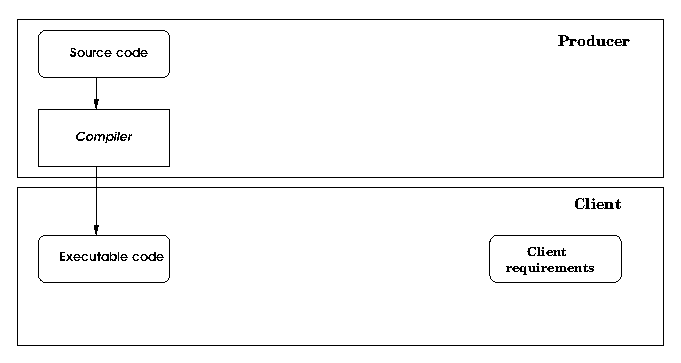
\epsfig{file=figs/mobileCode.eps}
%\caption{Mobile code}
\end{center}
%\end{frameit}
\end{figure} 
\end{frame}


%2.2
\begin{frame}[shrink,containsverbatim]
 \frametitle{What are the different approaches}
 \begin{itemize}
   \item type based verification  
        \begin{itemize}
               \item e.g. the bytecode verifier in the Java Virtual Machine (JVM) 
               \item only guarantees that the verified code does not corrupt  the JVM 
         \end{itemize}
   \item dynamic checks 
        \begin{itemize} 
                \item e.g. the sandbox mechanism in Java  % is this stack inspection mechanism
		\item runtime overhead  
        \end{itemize}
    \item program logic  verification 
         \begin{itemize} 
                \item e.g. verification tools like esc/java, Jack, Jive, Loop tool \ldots
                \item powerful, may verify for complex functional and security properties
	        \item however \ldots 
	 \end{itemize}
 \end{itemize}
\end{frame}

%2.1
\begin{frame}[shrink]
\frametitle{Source verification architecture}
\begin{figure} 
\begin{center}
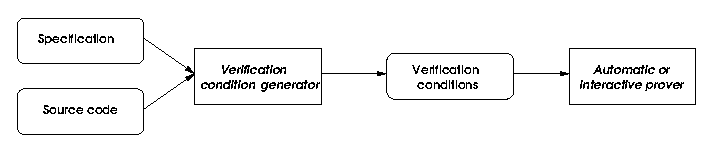
\epsfig{file=figs/sourceVerification.eps} % , width=5in, height=3in }
%\caption{Source verification architecture}
\end{center}
\end{figure}
\end{frame}





%2.3
\begin{frame}[shrink]
\frametitle{Mobile code verification}
\begin{figure}[hc]
\begin{center}
%
\includegraphics{bc.eps}
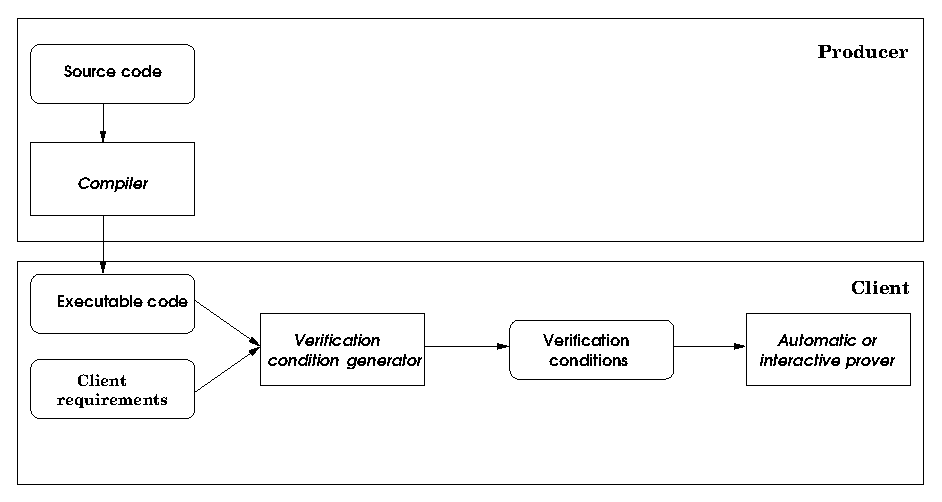
\epsfig{file=figs/mobileCodeVerif.eps}
%\caption{\sc Mobile code verification}
%\label{intro:mobileVerif}
\end{center}
\end{figure}
\end{frame}



%2.4
\begin{frame}[shrink]
\frametitle{Proof carrying code architecture for mobile code}
\begin{figure}[hc]
\begin{center}
%
\includegraphics{bc.eps}
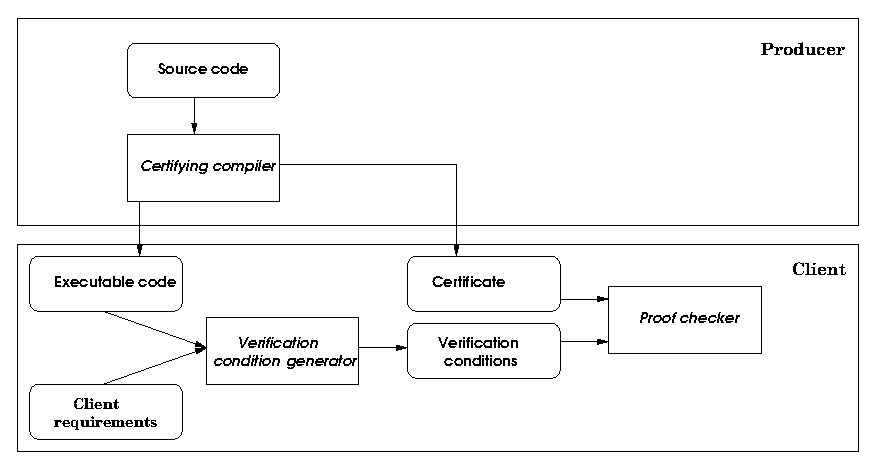
\epsfig{file=figs/PCC.eps}
%\caption{\sc Mobile code verification}
%\label{intro:mobileVerif}
\end{center}
\end{figure}
\end{frame}

%.2.5
\begin{frame}[shrink]
\frametitle{Proof preserving compilation for mobile code}
\begin{figure}[hc]
\begin{center}
%
\includegraphics{bc.eps}
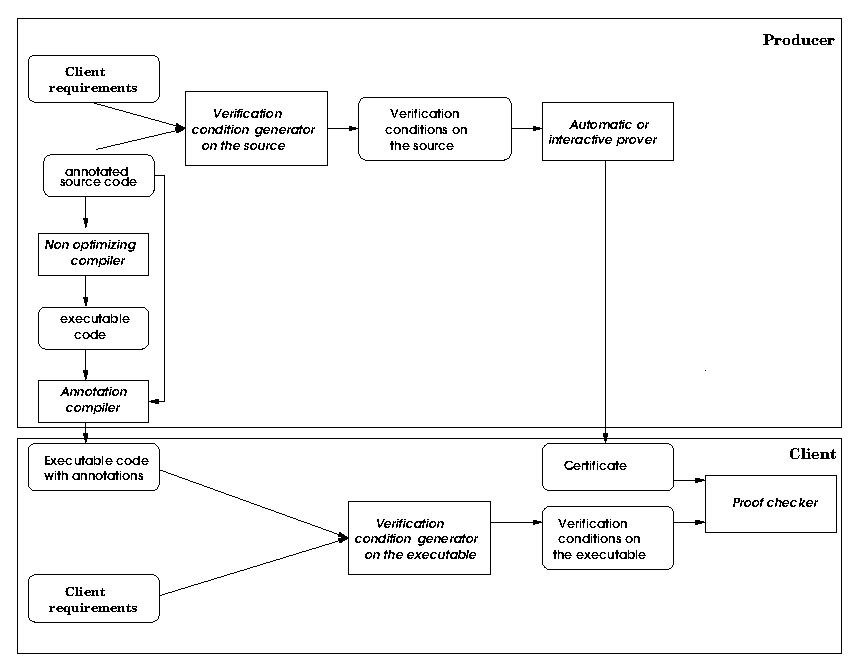
\epsfig{file=figs/PPO.eps}
%\caption{\sc Mobile code verification}
%\label{intro:mobileVerif}
\end{center}
\end{figure}
\end{frame}

\begin{frame}[shrink]
\frametitle{Approach}
\begin{figure}[hc]
\begin{center}
\begin{itemize} 
       \item Bytecode Modeling Language (BML)  
       \item a compiler from source annotations to bytecode annotations
       \item verification condition generator for bytecode  
       \item relation between verification conditions on source and non optimized bytecode    
             
\end{itemize}
\end{center}
\end{figure}
\end{frame}

%==================================================================================
%==========================BML=====================================================
%==================================================================================

\section{Bytecode Modeling Language}
\begin{frame}[shrink]
\frametitle{Why a specification language for bytecode?}
   \begin{itemize}
     \item PCC for complex policies 
     \item software audit which does not trust the compiler
     \item verification of programs which are directly written in a low level language
   \end{itemize}  
\end{frame}

\begin{frame}[shrink]\frametitle{Relation with JML}
  
  \begin{block}{Inspired by JML}
      JML is 
      \begin{itemize}
	  \item the defacto specification language for Java
	   \item expressive 
	\end{itemize}
  \end{block}

    inspired by the Java Modeling Language. Thus, supports most of the important features of JML
         \begin{itemize}
	    \item method preconditions
	     \item method postconditions
	      \item normal and exceptional behavior
	       \item assertions
	        \item loop invariants 
		 \item class invariants and history constraints 
	 \end{itemize}
        
\end{frame}


\begin{frame}[shrink]\frametitle{Design features}
\begin{itemize}
     \item Java compiler independent
     \item JVM compatibility
     \item corresponds to a partially desugared specification of BML
   
   \end{itemize} 
\end{frame}


\begin{frame}[shrink] \frametitle{Restrictions on the class file format}
\begin{itemize}
     \item \textbf{Line Number Table} and \textbf{Local Variable Table}  
     \item non optimized bytecode
 \end{itemize} 
\end{frame}

\begin{frame}[shrink]\frametitle{Compiler from JML to BML}
     \begin{itemize}
          \item Compilation of the Java source file 
	    \item Compilation of ghost variables
	      \item Desugaring of JML specification
		\item Linking phase
		  \item Locating the points for intra method specification 
		    \item Encoding the BML specification into user defined class attributes
       \end{itemize}
\end{frame}


\begin{frame}[fragile,shrink]\frametitle{Example}
\begin{columns}
\begin{column}{5.1cm}
{\tiny
\begin{lstlisting}[language=java]
//@ requires k >= 0 ;
//@ ensures \result == k*(k+1)/2;
public int sum (int k) {
  int sum = 0;		
  //@loop_modifies sum,i;
  //@loop_invariant i >= 0 && i<=k && 
  //@(sum == i*(i+1)/2);
  for  (int i = 0; i < k; i++ ) {
    sum = sum + i;
  } 	
  return sum;
}
\end{lstlisting}}
\end{column}

\begin{column}{5.1cm}
{\tiny
\begin{lstlisting}[language=jvmis]
//@requires lv[1] >= 0;
//@ensures result == lv[1]*(lv[1] + 1)/2;
Loop specification
//@atIndex 14 
//@modifies  lv[2], lv[3]
//@invariant lv[3]>=0 && lv[3]<=lv[1] &&
//@    lv[2]==lv[3]*(lv[3]+1)/2
0 iconst_0
1 istore_2
2 iconst_0
3 istore_3
4 goto 14 
7 iload_2
8 iload_3
9 iadd
10 istore_2 
11 iinc 3 
14 iload_3
15 iload_1
16 if_icmplt 7 
19 iload_2
20 ireturn
\end{lstlisting}}
\end{column}
\end{columns}

\end{frame}
%==================================================================================
%=================================VERIFICATION CONDITION GENERATOR=================
%==================================================================================


% verification condition generator for bytecode
\section{Verification condition generator for Java bytecode}
%\subsection{Overview of program verification}
\begin{frame}[shrink]
\frametitle{What is the problem of program verification ?}
\begin{block}{What do we verify?} 
 Program w.r.t.   program specification consisting of 
   \begin{itemize} 
       \item precondition %, which states the property that must have initial states    
       \item postcondition % which states the property that must hold when the method terminates
    \end{itemize}
\end{block}
\pause
\begin{block}{Partial correctness condition}
  A program \program~ respects a precondition \textit{Pre} and a 
 postcondition \textit{Post}  if for every initial state of  \program~ which satisfies \textit{Pre}
 if \program~ terminates, then \program~ terminates  in a state which  satisfies \textit{Post}
\end{block}
\end{frame}


  % why a verification condition generator
  % comparison with another possibilities for doing verification 
\begin{frame}\frametitle{Different techniques for program verification}
 \begin{itemize}
       \item perform the verification directly over the operational semantics
               \pause  \begin{itemize} 
                             \item  needs intensive user interaction
			\end{itemize}
                       \pause	
       \item use a Hoare style logic \pause 
                \begin{itemize} 
                        \item better than the previous approach, however still hard to automize 	
                \end{itemize}      
			  \pause	
       \item verification condition generator
                 \pause 
                \begin{itemize} 
                        \item an automatic procedure as far as the intermediate annotations are given  	     
               \end{itemize}
     \end{itemize}
\end{frame}
 

\begin{frame}
\frametitle{Bytecode verification condition generator}
\begin{itemize}
   \item generates verification conditions for every method separately
   \item works over the control flow graph of a method
   \item support for object manipulation, exceptions, method invokations, stack manipulation
   \item based on weakest precondition calculus
\end{itemize}
 \end{frame}



\begin{frame}[fragile,shrink]\frametitle{Weakest precondition predicate transformer for bytecode}
\begin{definition}
   $$\wpi:  nat \rightarrow \Method  \rightarrow \Pred $$
\end{definition}

\begin{block}{Rules}
   $$ \begin{array}{l}
        \wpi(i,\methodd ) = \\
         \wpi(i+1,\methodd)\subst{\counter}{\counter+1} \subst{\stack{\counter + 1}}{\locVar{k}}, \\
	  where \  \methodd[i] = \load \  \locVar{k} \\
	\\
	\wpi(i,\methodd ) = \\
       \stack{\counter - 1} \neq \Mynull \Rightarrow 
                            \wpi(i+1,\methodd)\subst{\stack{\counter}}{f(\stack{\counter} )} \\
			    \wedge \\ 
			     \stack{\counter - 1} \neq \Mynull \Rightarrow \methodd.\excPost( i, \NullPointerExc) \\
	  where \  \methodd[i] = \getfield \ f  \\
      \end{array}$$
\end{block}
\end{frame}


\begin{frame}[fragile,shrink]\frametitle{Example}
\begin{lstlisting}[language=jvmis]
method min
(*@\alert<10->{ \{ {\tiny $\locVar{1} \le \locVar{2} \wedge \locVar{1} > \locVar{2} \Rightarrow \locVar{1}  == \locVar{2} \wedge 
                          \locVar{1} > \locVar{2}    \wedge \locVar{1} \le \locVar{2} \Rightarrow \locVar{2} == \locVar{1} $} \}} @*)
   0: load 1
(*@\alert<9->{ \{ {\tiny $\stack{\counter } \le \locVar{2} \wedge \locVar{1} > \locVar{2} \Rightarrow \locVar{1}  == \locVar{2} \wedge 
                          \stack{\counter} > \locVar{2}    \wedge \locVar{1} \le \locVar{2} \Rightarrow \locVar{2} == \locVar{1} $} \}} @*)
   1: load 2
(*@\alert<8->{ \{ {\tiny $\stack{\counter - 1} \le \stack{\counter} \wedge \locVar{1} > \locVar{2} \Rightarrow \locVar{1}  == \locVar{2} \wedge 
                          \stack{\counter - 1} > \stack{\counter}    \wedge \locVar{1} \le \locVar{2} \Rightarrow \locVar{2} == \locVar{1} $} \}} @*)
   2: if_icmpgt 5
(*@\alert<7->{ \{ {\tiny $ \locVar{1} > \locVar{2} \Rightarrow \locVar{1}  == \locVar{2} \wedge 
		\locVar{1} \le \locVar{2} \Rightarrow \locVar{1} == \locVar{1} $} \}} @*)
   3: load 1
(*@\alert<6->{ \{ {\tiny $ \locVar{1} > \locVar{2} \Rightarrow \stack{\counter}== \locVar{2} \wedge 
		\locVar{1} \le \locVar{2} \Rightarrow   \stack{\counter} == \locVar{1} $} \}} @*)
   4: return
(*@\alert<5->{ \{ {\tiny $ \locVar{1} > \locVar{2} \Rightarrow \result == \locVar{2} \wedge 
		\locVar{1} \le \locVar{2} \Rightarrow \result == \locVar{1} $} \}} @*)

(*@\alert<4->{ \{ {\tiny $ \locVar{1} > \locVar{2} \Rightarrow \locVar{2}  == \locVar{2} \wedge 
		\locVar{1} \le \locVar{2} \Rightarrow \locVar{2} == \locVar{1} $} \}} @*)
   5: load 2
(*@\alert<3->{ \{ {\tiny $ \locVar{1} > \locVar{2} \Rightarrow \stack{\counter} == \locVar{2} \wedge 
		\locVar{1} \le \locVar{2} \Rightarrow \stack{\counter} == \locVar{1} $} \}} @*)
   6: return
(*@\alert<2->{ \{ {\tiny $ \locVar{1} > \locVar{2} \Rightarrow \result == \locVar{2} \wedge 
		\locVar{1} \le \locVar{2} \Rightarrow \result == \locVar{1} $} \}} @*)
\end{lstlisting}
\end{frame}

\begin{frame}\frametitle{Soundness of \wpi}
 \begin{definition}
If the verification conditions generated by \wpi~ over a bytecode program \program~ are 
valid formulas then \program~ is correct.
\end{definition}

The proof done w.r.t.  
\begin{itemize}
   \item a formalization of the operational semantics % $ \bcIns : state_1 \stateTrans state_2$
   \item interpretation of first order predicate formulas in a state 
   \item holds  for recursive methods
 \end{itemize}

\end{frame}


% how all these schemes are realised - the use of specification language
%%\frame{\frametitle{Components of the verification procedure}
% \begin{itemize}
%       \item specification of the application which expresses the intended behavior of the program
%                       
%       \item an algorithm for generating logical formulas whose validity implies the program correctness 
 %                     
%       \item a procedure for checking the validity of the verification conditions
%  \end{itemize}
%}
%%%%%%%%%%%%%%%%%%%%%%%%%%%%%%%%%%%%%%RELATION BTW BYTECODE AND SOURCE PROOF OBLIGATIONS %%%%%%%%%%%%%%%%%%%%%%%%%%%%%%%%%%%%%%%%%%%

 \section{Relation between bytecode and source verification conditions}


   \begin{frame}\frametitle{Motivations}
       \begin{itemize}
	  \item bytecode verification benefits from source verification 
          \item makes possible PCC for complex security and functional policies 
       \end{itemize}
   \end{frame}

   \begin{frame}\frametitle{The source language. Features}
       \begin{itemize}
	      \item  object manipulation and creation 
	   
              \item  runtime and userdefined exception throwing and handling
		
	       \item subroutines	
	    	
	      \item  method invokation
       \end{itemize}
   \end{frame}
   
 \begin{frame}\frametitle{Source weakest precondition calculus. Features}
    
	 \begin{block}{Rules}
	   \begin{itemize}
	      \item handles possible side effects
		{\tiny $$ \wpSrcStmt{ \var = \expressionSrc_2}{\normalPostSrc }{ \excPostSrc } =
                  \wpSrcExpr{\expressionSrc_2 }{ 
				    \normalPostSrc \subst{\var}{v}   
				   }{ \excPostSrc}{v} 
		  $$ } 
	      \item exceptional termination 
		{\tiny $$   \begin{array}{l}  \wpSrcExpr{\expressionSrc.\fieldd  }{\normalPostSrc }{ \excPostSrc }{v}  = \\
	                        \wpSrcExpr{\expressionSrc }{%\\
			                  % \phantom{wpiSr} 
                                             %\begin{array}{l} 
						        v_1 \neq \Mynull \Rightarrow \normalPostSrc \subst{v}{v_1.\fieldd} %\\
			                                \wedge% \\
						        v_1 = \Mynull \Rightarrow%\\
							 %\Myspace 
							 %\left( \begin{array}{l} 
							      % \forall \freshVar, 
							     % \neg \instances(\freshVar) \wedge \\
							       %\freshVar \neq \Mynull \Rightarrow%\\ 
							       \excPostSrc(\NullPointerExc ) %\subst{\EXC}{\freshVar}
							 % \end{array}\right)
							        
		                                 % \end{array}
						   }{% \\ 
                                          % \phantom{wpiSrc}
					    \excPostSrc }{v_1}  
				\end{array} $$ }
	      
	  \end{itemize}
    \end{block}
 \end{frame}

   \begin{frame}\frametitle{Compiler}

       \begin{itemize}
           \item non - optimizing 
           \item targets a stack based execution machine
	   %\item close to standard Java compilers 
       \end{itemize}
       Not so bad as  most of the Java compilers today are non optimizing  and  the result is relevant for the JVM 
   \end{frame}
  

   
    \begin{frame}[fragile,shrink]\frametitle{Compiler definition}

      {\small $$  \compile{ }_{\methodd} : nat * (\stmt \cup \expressionSrc ) \longrightarrow  list \ \bcIns * nat  $$}

      Most of the compilation rules are close to standard Java compilers:
      \begin{block}{Example for compilation rule}
     {\tiny $$  \begin{array}{l} \compileLabel{s}{ \newSrc \ \class  ( ) }{s+2}  = 
                 \begin{array}{l}
                       s :    \new \ \class; \\ 
		       s + 1: \dup; \\
		       s + 2 : \invoke \ \Constructor{\class};     
	       \end{array} \end{array} $$}
      \end{block}

      Specific features:
      \begin{block}{Loop compilation}
       {\tiny  $$\compileLabel{s}{\while \ (\expressionSrcRel) \lbrack \invariant, \modLoop \rbrack \ \do \ \{ \stmt \} }{e} = 
         \begin{array}{l}
              s: \goto \ e' + 1; \\
	      \compileLabel{s +  1}{\stmt}{e' }; \\
	     % \lbrack  \compileSynt{\invariant} , \compileSynt{\modLoop} \rbrack \\ 
	      \compileLabel{e' +  1}{\expressionSrcRel}{e  -1 };\\
	      e: \ifCond \ s +  1; \\
	      \\\\
	      \addLoopTable{\methodd}{e'+1}{\invariant }{\modLoop}
	 \end{array} $$}
      \end{block}
\end{frame}




\begin{frame}[fragile,shrink]\frametitle{Properties of the compiler function}
  \begin{itemize}
     
     \item compilation of a statement (expressions) may contain instructions which either target instructions inside the compilation of a statement or  the 
           first instruction of the next statement, if there is next statement 
     
     \item expressions are compiled into a sequence of instructions which does not contains jumps 
     
     %\item substatement relation preserved by the compiler (Properties \ref{compile:prop:compPropSubstmt}, \ref{compile:prop:compProp6}).

     \item a compilation of a source statement contains cycles only if the source statement contains cycles 
     
     \item exception handler preservation 
     
  \end{itemize}
\end{frame}

\begin{frame}[fragile,shrink]\frametitle{Equivalence of proof obligations.Example}

\begin{block}
  {\small \begin{tabular}{lll} 
   $ \compileLabel{i}{ \lstinline!sqr + 2*s ! }{i+4}$ & = &
   \begin{tabular}{l} 
     $\compileLabel{i}{ \lstinline!sqr! }{i}$ \\
     $\compileLabel{i+1}{ \lstinline!2*s! }{i+3} $\\
     \lstinline!i+4: add!
      \end{tabular} \\
      where & & \\
      $\compileLabel{i}{ \lstinline!sqr! }{i}$ & = & \lstinline! i: load sqr!\\
      \\
      $\compileLabel{i+1}{ \lstinline!2*s! }{i+3}$ & = &
      \begin{tabular}{l} 
        % \lstinline!i  : load sqr! \\
	 \lstinline!i+1: const 2!  \\
	 \lstinline!i+2: load s!   \\
	 \lstinline!i+3: mul!	   \\
	 %\lstinline!i+4: add!	    
   \end{tabular}
    \end{tabular}
}
\end{block}


%\begin{block}
  {\small
  $$  \begin{array}{ll}
         1.1   &     \alert<7->{ \mbox{\rm \lstinline!sqr!} + \mbox{\rm \lstinline!2!}*\mbox{\rm \lstinline!s!} = \mbox{\rm \lstinline!5!}   } \\ 
         1.2   &   \lstinline!i:  load sqr!  \\
         1.3   &     \alert<6->{  \stack{\counter} + \mbox{\rm \lstinline!2!}*\mbox{\rm \lstinline!s!} = \mbox{\rm \lstinline! 5!}   }\\
         1.4   &   \lstinline!i+1: const 2!	  \\
	 1.5   &     \alert<5->{   \stack{\counter - 1} + \stack{\counter } *\mbox{\rm \lstinline!s!} = \mbox{\rm \lstinline! 5!}    }\\
	 1.6   &   \lstinline!i+2: load s!	  \\
	 1.7   &     \alert<4->{   \stack{\counter - 2}  + \stack{\counter - 1} * \stack{\counter} = \mbox{\rm \lstinline! 5!}    }\\
	 1.8   &   \lstinline!i+3: mul!	          \\
	 1.9   &     \alert<3->{  \stack{\counter - 1}  + \stack{\counter} = \mbox{\rm \lstinline! 5!}   }\\
	 1.10  &   \lstinline!i+4: add!	          \\
	 1.11  &     \alert<2->{  \stack{\counter} = \mbox{\rm \lstinline! 5 !}    } \\       
               & \\
	       & \\
  %\end{array}$$}

%\end{block}



  % \begin{Example} {
  %{\small $$\begin{array}{ll}
      2.1   &    \wpSrcExpr{\lstinline!sqr + 2*s ! }{\alert<2->{ v = 5} }{\excPostExpl}{v} =   \\
      2.2   &  	 \wpSrcExpr{\lstinline!sqr!}{\wpSrcExpr{\lstinline!2*s ! } { \alert<3->{ (v=5)\subst{v}{v_{sqr} + v_{2*s}} } }{\excPostExpl}{v_{2*s}}  }{\excPostExpl}{v_{sqr}} =   \\
      2.3   & 	 \wpSrcExpr{\lstinline!sqr!}{\wpSrcExpr{\lstinline!2! }{\wpSrcExpr{\lstinline!s! }{ \alert<4->{ (v_{sqr}+v_{2*s}=5)\subst{v_{2*s}}{v_{2}*v_{s}}} }{\excPostExpl}{v_{s}}  }{\excPostExpl}{v_{2}} }{\excPostExpl}{v_{sqr}} =   \\
      2.4   &	 \wpSrcExpr{\lstinline!sqr!}{\wpSrcExpr{\lstinline!2! }{\alert<5->{ (v_{sqr} + v_{2}*v_{s}=5 ) \subst{v_{s}}{s}} }{\excPostExpl}{v_{2}} }{\excPostExpl}{v_{sqr}} =   \\
      2.5   &    \wpSrcExpr{\lstinline!sqr!}{\alert<6->{(v_{sqr} + v_{2}*\lstinline!s!=5 ) \subst{v_{2}}{2} } } {\excPostExpl}{v_{sqr}} =   \\
      %2.6   &	 (v_{sqr} + 2*\lstinline!s!=5 ) \subst{v_{sqr}}{\lstinline!sqr!  } =   \\
      2.6   & \alert<7->{  \lstinline!sqr! + 2*\lstinline!s!=5  }
\end{array}$$
} %}  \end{Example}

\end{frame}

%%%%%%%%%%%%%%%%%%%%%%%%%%%%%%%%%%%%%%RELATION BTW BYTECODE AND SOURCE PROOF OBLIGATIONS %%%%%%%%%%%%%%%%%%%%%%%%%%%%%%%%%%%%%%%%%%%
 \section{Applications}
 \subsection{Java-to-Native Compilation}


\begin{frame}[shrink]\frametitle{Java-to-Native Compilation}
Compiling Java bytecode into native code brings runtime advantages:
\begin{itemize}
    \item Faster execution
    \item Especially beneficial for restrained systems with non-sophisticated JVMs
\end{itemize}
But Java-to-Native compilation also comes with drawbacks:
\begin{itemize}
    \item Native code is typically 3 to 4 times bigger than bytecode,
\end{itemize}
\end{frame}

\begin{frame}[fragile]\frametitle{Why is Native Code so Huge? An Example}
The \emph{idiv} bytecode throws an \texttt{ArithmeticException} if the divisor is equal to zero:

\begin{columns}
\begin{column}{5.1cm}
\begin{lstlisting}[language=jvmis]
iload i
iload j
idiv
ireturn
\end{lstlisting}
\end{column}
\begin{column}{5.1cm}
\begin{lstlisting}[language=C]
int i, j;
(*@\alert<2->{if (j == 0)}@*)
	(*@\alert<2->{THROW(ArithmeticException);}@*)
RETURN_INT(i / j);
\end{lstlisting}
\end{column}
\end{columns}
\bigskip
There are many checks of this kind:
\begin{itemize}
\item Checking a pointer is not \emph{null} before dereferencing it,
\item Checking an array is accessed inside its bounds,
\item Checking an array is created with a positive size,
\item Checking affected types are compatible,
\item ...
\end{itemize}
SPECjvm98: 2964 exception check sites for a native size of 23598 bytes (Ishizaki et al.).
\end{frame}


\begin{frame}\frametitle{Possible Times for Compilation}
Java-to-Native compilation is typically done at two moments:

\textbf{Ahead-Of-Time:}
\begin{itemize}
\item Performed off-board,
\item Methods to compile must be selected in advance,
\item No or little time constraints,
\item Native code replaces the bytecode,
\end{itemize}

\textbf{Just-In-Time:}
\begin{itemize}
\item Performed by an on-board compiler,
\item Methods to compile are chosen by the JVM,
\item Little time to perform optimizations,
\item Native code must be stored in writable memory in addition to the bytecode
\end{itemize}

In either cases, the runtime exceptions check sites must be issued.
\end{frame}




\begin{frame}\frametitle{Suppressing Exceptions Check Sites using formal verification}

Runtime exceptions are (usually) a safety against programming errors. They should not be triggered by sane code.

We propose to formally prove that runtime exceptions are never thrown by a program.

Methodology:
\begin{enumerate}
\item Annotate source code with JML specification to express that no runtime exception will be thrown
\item Compile JML specification into BML as user-defined class file attributes
\item Generate and prove verification conditions over the bytecode and BML
\item Annotate class files with useless runtime exception check sites attribute
\end{enumerate}
\end{frame}

% \frame{[fragile]
%\frametitle{Annotating Source with JML}
%
%Write annotations that express no runtime exception is thrown.
%\begin{lstlisting}[language=java]
%private/*@spec_public */short tab[];
%//@requires size <= tab.length && tab != null;
%//@ensures true;
%//@exsures (Exception) false;
%public void clear(int size) {
%  int code;
%  //@loop_modifies code, tab[*];
%  //@loop_invariant code <= size && code >= 0;
%  for (code = 0; code < size; code++) {
%    tab[code] = 0;
%  }
%}
%\end{lstlisting}
%
%\only<1>{Lines 2 and 3 specifies what the method requires from its callers}
%\only<2>{Lines 4 and 5 specifies what the method guarantees to its callers}
%\only<3>{Lines 8 and 9 specifies the loop invariants}
%}

\begin{frame}[fragile]
\frametitle{Compile JML annotations into BML attributes}

Class files are enriched with a user-defined BML attribute that expresses the JML specification.

\begin{lstlisting}[language=jvmis]
//@ requires tab(lv[0]) != null;
//@ requires lv[1] <= length(tab(lv[0]));
//@ ensures true;
//@ exsures (Exception) false;

method clear
  iconst_0
  istore_2
  ...
  return
\end{lstlisting}
\end{frame}

% \frame{
%\frametitle{Optimizing the Native Code}
%
%When a runtime exception throwing bytecode is met by the compiler, the useless exception sites attribute is checked with the bytecode index to see if the exception site is needed.
%
%\begin{itemize}
%\item Cheap and efficient for both ahead-of-time and just-in-time compilations
%\item The annotations must be trusted!
%\end{itemize}
%}

\begin{frame}
\frametitle{Experimental Results}
\begin{center}
  Number of necessary exception check sites

  \bigskip
  \begin{tabular}{|l|r@{\extracolsep{0.2cm}}rr|}
    \hline
    \multirow{2}*{Program} & \multicolumn{3}{c|}{\# of exception check sites} \\
    \cline{2-4} & Bytecode & ~~~~~~JC & Proven AOT\\
    \hline
    \benchname{crypt} & 190 & 79 & 1\\
    \benchname{banking} & 170 & 12 & 0\\
    \benchname{scheduler} & 215 & 25 & 0\\
    \benchname{tcpip} & 1893 & 288 & 0\\
    \hline
  \end{tabular}
  \bigskip
  \begin{tabular}{|l|r@{\extracolsep{0.2cm}}rr|}
    \hline
    \multirow{2}*{Program} &  \multicolumn{3}{c|}{Memory footprint (bytes)}\\
    \cline{2-4} & Bytecode & Naive AOT & Proven AOT\\
    \hline
    \benchname{crypt} & 1256 & 5330 & 1592\\
    \benchname{banking} & 2320 & 5634 & 3582\\
    \benchname{scheduler} & 2208 & 5416 & 2504\\
    \benchname{tcpip} & 15497 & 41540 & 18064\\
    \hline
  \end{tabular}
\end{center}
\end{frame}


\subsection{Constraint memory consumption policies using program logic}

\begin{frame}
\frametitle{Security and TPD}
   Trusted Personal Devices (TPD) rely on platform independent execution frameworks - JVM, CLR.
   Java provides:
       \begin{itemize}  
	   \item  memory access control - stack inspection
	    \item bytecode verification - static type checking
	     \item \alert{no control over resource usage }
	 \end{itemize}
\end{frame}

\begin{frame} \frametitle{Solutions }

\begin{itemize}
     \item Static Analysis and Abstract Interpretation
        \begin{itemize}
	  \item analysis performed on an abstraction of the program
	  \item not precise
	\end{itemize}
	\pause
     \item Proof Carrying code 
        \begin{itemize}
	  \item fully automated (certifying  compiler)
	  \item not precise
        \end{itemize}
        \pause
     \item Runtime Checks 
        \begin{itemize}
	  \item precise 
	  \item runtime overhead
	\end{itemize}
\end{itemize}
\end{frame}


\begin{frame}
\frametitle{Alternative solution for the constraint memory usage policy for Java Bytecode}

    \begin{block}<+->{ Specification }
     \begin{itemize}
       
       \item \uncover<1->{  part of the specification provided by the producer}
	 \uncover<2->{ \alert{- for the sake of preciseness}}
 
    \end{itemize}
   \end{block}

  \begin{block}<3->{Floyd-Hoare style logic }
     \begin{itemize}
           \item \uncover<3->{verification condition generator for Java bytecode} \uncover<4->{ \alert{- independent from the source code}}
           \item  \uncover<3->{ checks done statically }\uncover<5->{ \alert{- no runtime overhead}}
           
    \end{itemize}
   \end{block}
\end{frame}

\begin{frame}[containsverbatim] \frametitle{Modeling the memory heap}  
  \begin{block}<+->{Used heap space is a ghost variable}
    \begin{verbatim} //@ public ghost static int Mem \end{verbatim}
  \end{block}
  

  \begin{block}<1->{ The upper bound of the memory space that can be used is a model variable}
    \begin{verbatim} //@ public ghost static int Max \end{verbatim}   
  \end{block}
\end{frame}


\begin{frame}[containsverbatim,shrink] \frametitle{Principles for specifying memory allocations}
  \begin{Example} {
    \begin{lstlisting}[language=jvmis]
      method m
         new A
         //@set Mem = Mem+memUnit(A)
         dup
         invokevirtual A
    \end{lstlisting}
 }   
  \end{Example} 
  
  \begin{block}<+->{The $wp$ rule for the set specification construction }
     $wp(\verb!set Mem = M! , \psi , \psi') = \psi[\verb!Mem! \leftarrow \verb!M!] $
  \end{block}
\end{frame}

\begin{frame} \frametitle{Specifying methods}
  \begin{block}<+->{Method Specification}
    \begin{itemize}
      \item  <1->{ expresses the fact that the method does not break the bounded memory consumption policy }
      
      \item  <2->{  assume in the precondition that  when method starts execution the application has consumed so much memory units such that the method execution 
 will not break the memory consumption restrictions}
      \item  <3->{ guarantee postcondition -  when method ends execution it should have consumed not more than what it has assumed in the precondition  }
     \end{itemize}
  \end{block}
\end{frame}

\begin{frame}[fragile,shrink]\frametitle{Principles. Specifying Methods}
  \begin{Example}{
      \begin{lstlisting}[language=jvmis]
      //@requires Mem+memUnit(A)+
      //@            methCons(init_A)<=Max
      //@ensures Mem<=old(Mem)+
      //@           memUnit(A)+methCons(init_A)
      method m
         new A
         //@set Mem = Mem+memUnit(A)
         dup
         invokevirtual A
      \end{lstlisting}         
       }
  \end{Example} 
\end{frame}


%13
\begin{frame}[fragile,shrink]\frametitle{Principles. Loops}
 \begin{Example}{ {\tiny 
 \begin{lstlisting}[language=jvmis]
//@requires Mem + iter*( memUnit(A) + methCons(init_A)) <= Max
//@ensures Mem <= \old(Mem) +   iter*(memUnit(A) +  methCons(init_A))   
 method m(int iter)
  //@ghost int MemL
  //@set MemL = Mem
  Loop specification
  (*@\textsf{atIndex:}@*)16
  (*@\textsf{modifies}:@*)Mem, i
  (*@\textsf{invariant}:@*) Mem <= MemL + i*(memUnit(A) + methCons(init_A)) && i <= iter
  (*@\textsf{variant:}@*) iter-i
  0 const 0
  1 store i
  2 goto 16 
  5 new A
  //@set Mem=Mem+memUnit(A);
  8 dup
  9 invokespecial init_A
  12 store a
  13 iinc i
  16 load i
  17 load iter
  18 if_icmplt 5 
  21 return
 \end{lstlisting}}  
}\end{Example} 
\end{frame}
  
 \section{Future work}
     \subsection{Results}
\begin{frame}[fragile,shrink]\frametitle{Future directions. Verification condition generator}
         \begin{itemize}
	   \item Improvement of the verification condition generator 
              \begin{itemize}
	           \item use of a two dimensional heap which allows to quantify over fields 
               \end{itemize}
	    \item Extension of the verification condition generator 
                 \begin{itemize}
	             \item   multithreading
		  \end{itemize}
          \end{itemize}
\end{frame}

\begin{frame}[fragile,shrink]\frametitle{Future directions. Property coverage  }
	   
                  \begin{itemize}
	                \item pure methods 
			  \item alias control
			  \item modular verification of class invariants
			    
		   \end{itemize}  

\end{frame}

\begin{frame}[fragile,shrink]\frametitle{Future directions. Relation between source and bytecode verification}
		
		     \begin{itemize}
	                 \item non optimizing compilation - 
                           \begin{itemize}
	                      \item verification conditions on bytecode and source equivalent modulo names and types
                               \item extension of the verification condition generator 
			       for overcoming these differences
			    \end{itemize}
			   
			  \item optimizing compilation - how to transform certificates from 
                    \end{itemize}
           

\end{frame}

\begin{frame}[fragile,shrink]\frametitle{Future directions.Towards a PCC framework  }
		     \begin{itemize}
	                \item certificate format - small and easily checked 
			  \item hybrid certificates
		     \end{itemize}
          
\end{frame}

\begin{frame}[fragile,shrink]\frametitle{Future directions. PCC. Light weight verification condition generator }
		     \begin{itemize}
                          \item  certificate generation on the producer site - no constraints on the computational resources used
			    \item certificate checking on the  client site - should use few computational resources
			      \item both sites use a verification condition generator
		       \end{itemize}
                     

\begin{figure}[hc]
\begin{center}
%
\includegraphics{bc.eps}
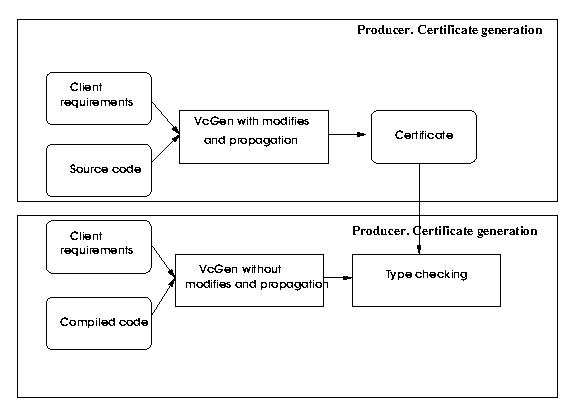
\epsfig{file=figs/VCefficient.eps}
%\caption{\sc Mobile code verification}
%\label{intro:mobileVerif}
\end{center}
\end{figure}

\end{frame}
\end{document}

